\section{Research Plan}

\subsection{Overview}

\begin{figure}[t]
\centering
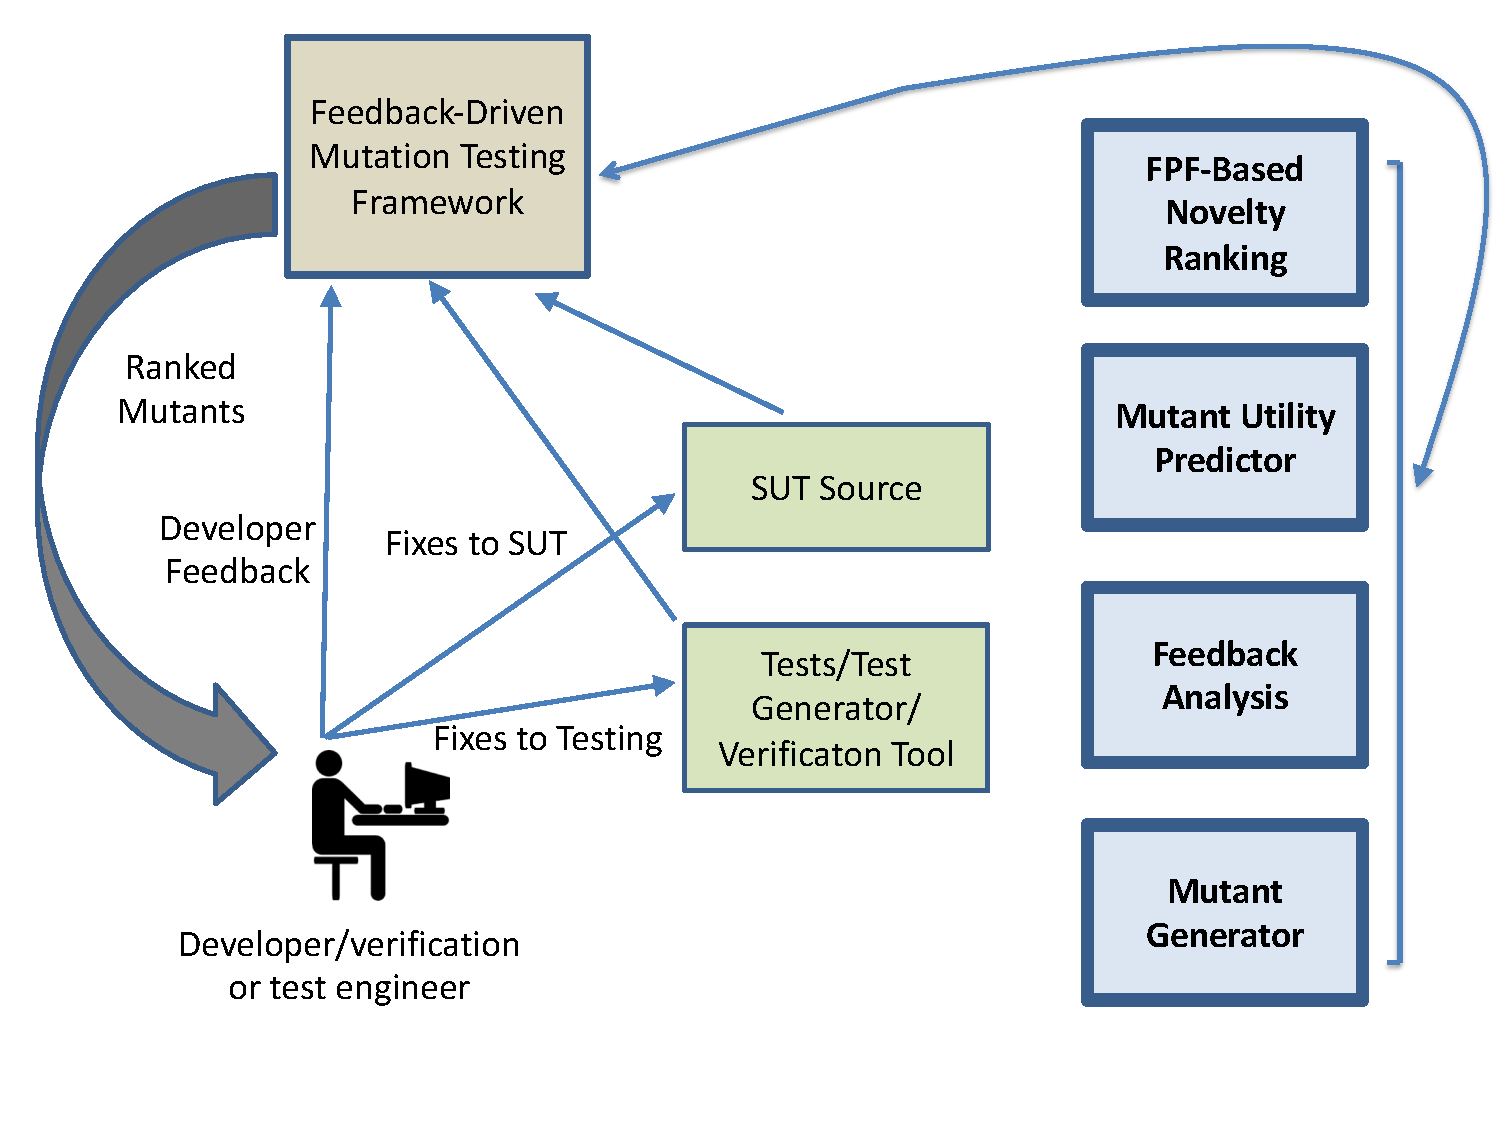
\includegraphics[width=0.8\columnwidth]{TestFlow}

\caption{Basic flow of feedback-driven mutation testing.}
\label{fig:flow}
\end{figure}

Figure \ref{fig:flow} shows the basic outline of a proposed workflow
and components needed to support feedback-driven mutation testing.
These components serve to organize our research plan.


\subsubsection{FPF-Based Novelty Ranking}
\label{sec:fpfplan}

Ranking unkilled mutants according to how much ``new'' information they might
provide to users requires more than simply using the FPF algorithm.
FPF requires a distance metric, and a distance metric requires a
\emph{representation} of mutants.  Mutants can be similar because they
modify the same line, function, class, or module, but also because,
despite being located in very different parts of a program, they are
very semantically similar.  E.g., a mutant to the parser of a compiler, to
an I/O error-handling routine in the code generator, and to a complex
optimization pass may all be very ``similar'' in the only meaningful
sense if all three mutants modify logging statements that don't have
any actual effect on the state of the compiler.  Figure
\ref{fig:distances} shows the fundamental problem.  Elements of the
distance metric must include mutant location, mutation operator, and
some representation of the code element modified --- language
construct, functions called, variables modified, and so forth.  This
is a complex problem in representation and weighting of elements of a
representation, especially if we aim at producing a language and
project agnostic metric, perhaps one open to tuning via feedback
analysis.  We plan to exploit metric learning
methods~\cite{kulis2012metric}, but are aware that to avoid over-fitting
to even a set of good examples, the final metric may have to be
hand-tuned.  In part this is due to the difficulty of establishing
large amounts of ground truth data; although there are unsupervised
approaches to metric learning~\cite{scholkopf1998nonlinear,tipping1999probabilistic}, the most popular approaches require supervision.

\subsubsection{Mutant Utility Predictor}

\subsubsection{Feedback Analysis}

\subsubsection{Mutant Generator}

\subsection{Core Research Questions}

\subsubsection{Research Questions for Feedback-Driven Mutation Testing
in General}

\begin{enumerate}
\item How can we form a generalized, language-agnostic representation
  of and distance metric for program mutants for use in FPF?
\item How can we incorporate feedback from users into the
  representation and distance metric?
\item How can we balance FPF-based selection of mutants for novelty
  with predictions of mutant equivalence, outcome, dominance, and
  productivity?
\item How can we identify outliers in otherwise similar groups of
  mutants, and is such identification useful?
\item How can we set budgets for automated test generation and
  timeouts for verification efforts to quickly estimate whether a
  mutant is killable?
\item Can we predict whether a mutant's unkillability is due to poor test 
  generation  or due to oracle weakness? 
\item How can we most effectively use already generated killing tests
  and counterexamples to prune mutants?
\item Is distance-based clustering plus timing information useful for quickly
  eliminating killable mutants similar to already-killed mutants?  How
  does this relate to Predictive Mutation Testing (PMT)?

\end{enumerate}

\subsubsection{Research Questions Specific to Any-Language Mutation}

\begin{enumerate}
\item How can we maximize the efficiency and usability of a
  fundamentally language-agnostic regular-expression-based approach to
  mutant generation?
\item How can we extend the language of regular expressions to allow
  for language-agnostic definition of mutation operators that require
  more parsing-like analysis of code structure, without compromising
  the usability and simplicity of the approach?
\item Is it possible to perform on-the-fly mutant generation for very
  large projects, and reconcile this approach with FPF (e.g., generate
  new mutants with, possibly approximate, desired distances from
  already evaluated mutants)?
\end{enumerate}

\subsection{Work and Evaluation Plans}
\label{sec:workplan}
\subsection{Evaluation Plan}
